%% -*- coding: utf-8 -*-
\documentclass[12pt,pagesize,paper=192mm:108mm]{scrbook} 
%1920x1080 1280x720
\areaset[current]{192mm}{108mm}
\usepackage{calc}
\usepackage[T2A]{fontenc}
\usepackage[utf8]{inputenc}
\usepackage[english,russian]{babel}
\usepackage{microtype}
\usepackage{misccorr}
\usepackage{cmap}
%\usepackage[unicode=true]{hyperref}
\usepackage{graphicx}
\usepackage{amssymb}
\usepackage{amsmath}
%\usepackage{srcltx}
\usepackage{textcomp}
\usepackage{xspace}
%научные символы и смайлики \smiley \frownie
\usepackage{wasysym}
\usepackage{ccicons}
\begin{document}
\begin{titlepage}
  \vspace*{-1em}
  \begin{center}
    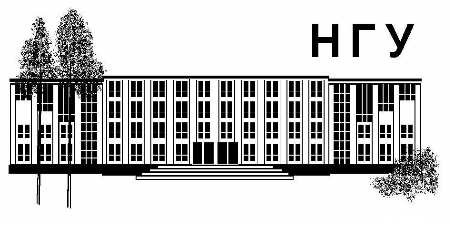
\includegraphics[width=0.2\textwidth]{../NSU-logo}

    Кафедра теоретической физики физического факультета НГУ
 %   \medskip

    \Large
    Профессор Фадин В.\,С.

    \huge
    \textbf{Теория сильных взаимодействий}
%    \smallskip
    
    \Large
    Лекция № 10
    \vfill
    
    \normalsize
    \begin{minipage}{0.95\linewidth}
      \small Константы связи в КЭД и КХД. Адронный тензор $W_{\mu\nu}$ и его
      представление через коммутатор токов. Область вблизи светового
      конуса. Операторное разложение. Особенности вильсоновских
      коэффициентов. Твист оператора. Операторы твиста два. Связь
      тензора $W_{\mu\nu}$ с амплитудой $T_{\mu\nu}$. Дисперсионный
      интеграл для $T_{\mu\nu}$ и связь с моментами структурных
      функций $(F_{1,2})$. Матричные элементы локальных операторов и
      их зависимость от $\mu$. Мультипликативная перенормировка
      операторов. Уравнение ренорм"=группы. Аномальная размерность
      операторов. Зависимость вильсоновских коэффициентов от
      $Q^2$. Смешивание синглетных операторов при
      перенормировке. Связь аномальных размерностей с моментами ядер
      Альтарелли"--~Паризи.
    \end{minipage}
    \vfill
    
    \normalsize \ccbysa\hspace{0.5em}   Новосибирск 2014   
  \end{center}
\end{titlepage}
\end{document}
